%===================================================================================================================
%                                             TABLES
%===================================================================================================================
%-------------------------------------------------------------------------------------------------------------------
%
%-------------------------------------------------------------------------------------------------------------------
%\begin{table*}[t]\scriptsize
%\caption{
%Results from the Markov chain Monte Carlo (MCMC) sampling applied to the mixed model fitted to the correlation data.
%The column ``Estimate'' represent the model estimates. % for each level of the parameter of the model.
%The next 3~columns represent the Highest Posterior Density (HPD) intervals (mean, upper and lower band of the $95\%$ confidence interval) of the MCMC samples.
%The last column shows the MCMC generated p-values, the symbol $^{*}$ denotes statistical significance below 0.01.
%}
%\label{table:pValsCorr}
%\centering
%%\begin{tabular}{c c c c c c}
%\begin{tabular}{l r r r r l}
%\toprule
% & Estimate & MCMCmean & HPD95lower & HPD95upper & pMCMC \tabularnewline
%\toprule
%(Intercept) &  0.801071 &  0.801008 &  0.760609 &  0.842671 & 0.00002$^{*}$ \tabularnewline
%  hybrid-10Hz - hybrid-15Hz & -0.015898 & -0.015843 & -0.029056 & -0.002668 & 0.01892 \tabularnewline
%  hybrid-10Hz - hybrid-8.57Hz & -0.003925 & -0.003845 & -0.017088 &  0.009328 & 0.57244 \tabularnewline
%  hybrid-12Hz - hybrid-15Hz & -0.000273 & -0.000278 & -0.013391 &  0.012947 & 0.97272 \tabularnewline
%  hybrid-12Hz - hybrid-8.57Hz &  0.001052 &  0.001075 & -0.012065 &  0.014290 & 0.87228 \tabularnewline
%  hybrid-15Hz - hybrid-8.57Hz & -0.013637 & -0.013633 & -0.026976 & -0.000630 & 0.04344 \tabularnewline
%  oddball - hybrid-10Hz & -0.128680 & -0.128632 & -0.141867 & -0.115555 & 0.00002$^{*}$ \tabularnewline
%  oddball - hybrid-12Hz & -0.104052 & -0.104029 & -0.116998 & -0.090586 & 0.00002$^{*}$ \tabularnewline
%  oddball - hybrid-15Hz & -0.088516 & -0.088469 & -0.101964 & -0.075437 & 0.00002$^{*}$ \tabularnewline
%  oddball - hybrid-8.57Hz & -0.108974 & -0.108927 & -0.122265 & -0.095920 & 0.00002$^{*}$ \tabularnewline
%%(Intercept) &  0.7798 &  0.7794 &  0.7378 &  0.8241 & 0.0002$^{*}$\tabularnewline
%%  hybrid-10Hz - hybrid-15Hz & -0.0131 & -0.0131 & -0.0257 &  0.0000 & 0.0456\tabularnewline
%%  hybrid-10Hz - hybrid-8.57Hz & -0.0083 & -0.0082 & -0.0205 &  0.0046 & 0.2124 \tabularnewline
%%  hybrid-12Hz - hybrid-15Hz &  0.0002 &  0.0003 & -0.0131 &  0.0128 & 0.9604 \tabularnewline
%%  hybrid-12Hz - hybrid-8.57Hz &  0.0023 &  0.0023 & -0.0100 &  0.0150 & 0.7336 \tabularnewline
%%  hybrid-15Hz - hybrid-8.57Hz & -0.0097 & -0.0096 & -0.0222 &  0.0032 & 0.1456 \tabularnewline
%%  oddball - hybrid-10Hz & -0.1354 & -0.1354 & -0.1483 & -0.1230 & 0.0002$^{*}$ \tabularnewline
%%  oddball - hybrid-12Hz & -0.1062 & -0.1060 & -0.1190 & -0.0936 & 0.0002$^{*}$ \tabularnewline
%%  oddball - hybrid-15Hz & -0.0909 & -0.0907 & -0.1030 & -0.0773 & 0.0002$^{*}$ \tabularnewline
%%  oddball - hybrid-8.57Hz & -0.1122 & -0.1121 & -0.1249 & -0.0988 & 0.0002$^{*}$ \tabularnewline
%\bottomrule
%\end{tabular}
%\end{table*}

%===================================================================================================================
%                                             FIGURES
%===================================================================================================================
\clearpage

%-------------------------------------------------------------------------------------------------------------------
%
%-------------------------------------------------------------------------------------------------------------------
\begin{figure}[t]
\centering
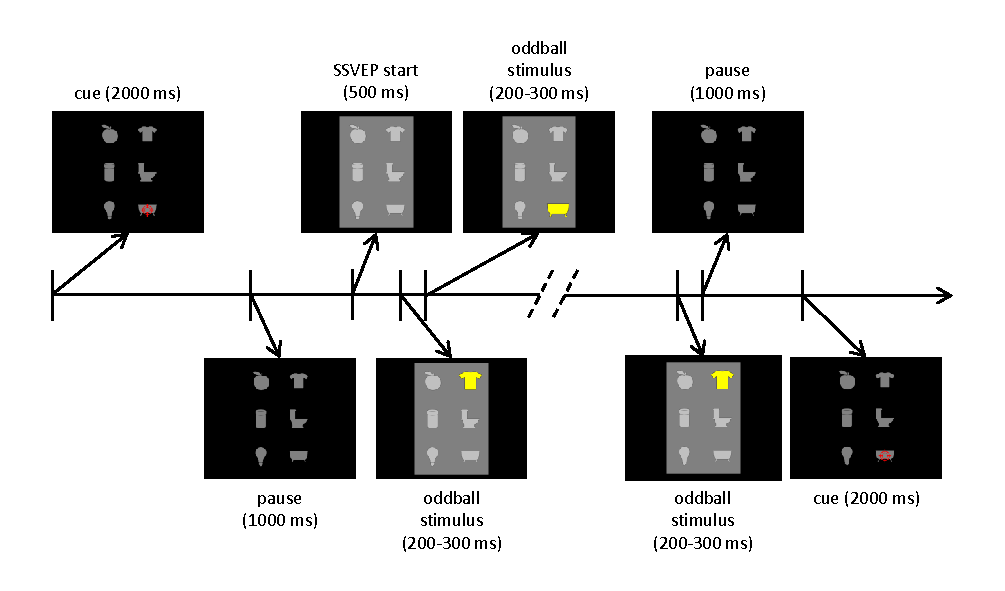
\includegraphics{pix/stimulationSequence2}
\caption{stimulation sequence}
\label{fig:stimSeq}
\end{figure}

%-------------------------------------------------------------------------------------------------------------------
%
%-------------------------------------------------------------------------------------------------------------------
\begin{figure}[t]
\centering
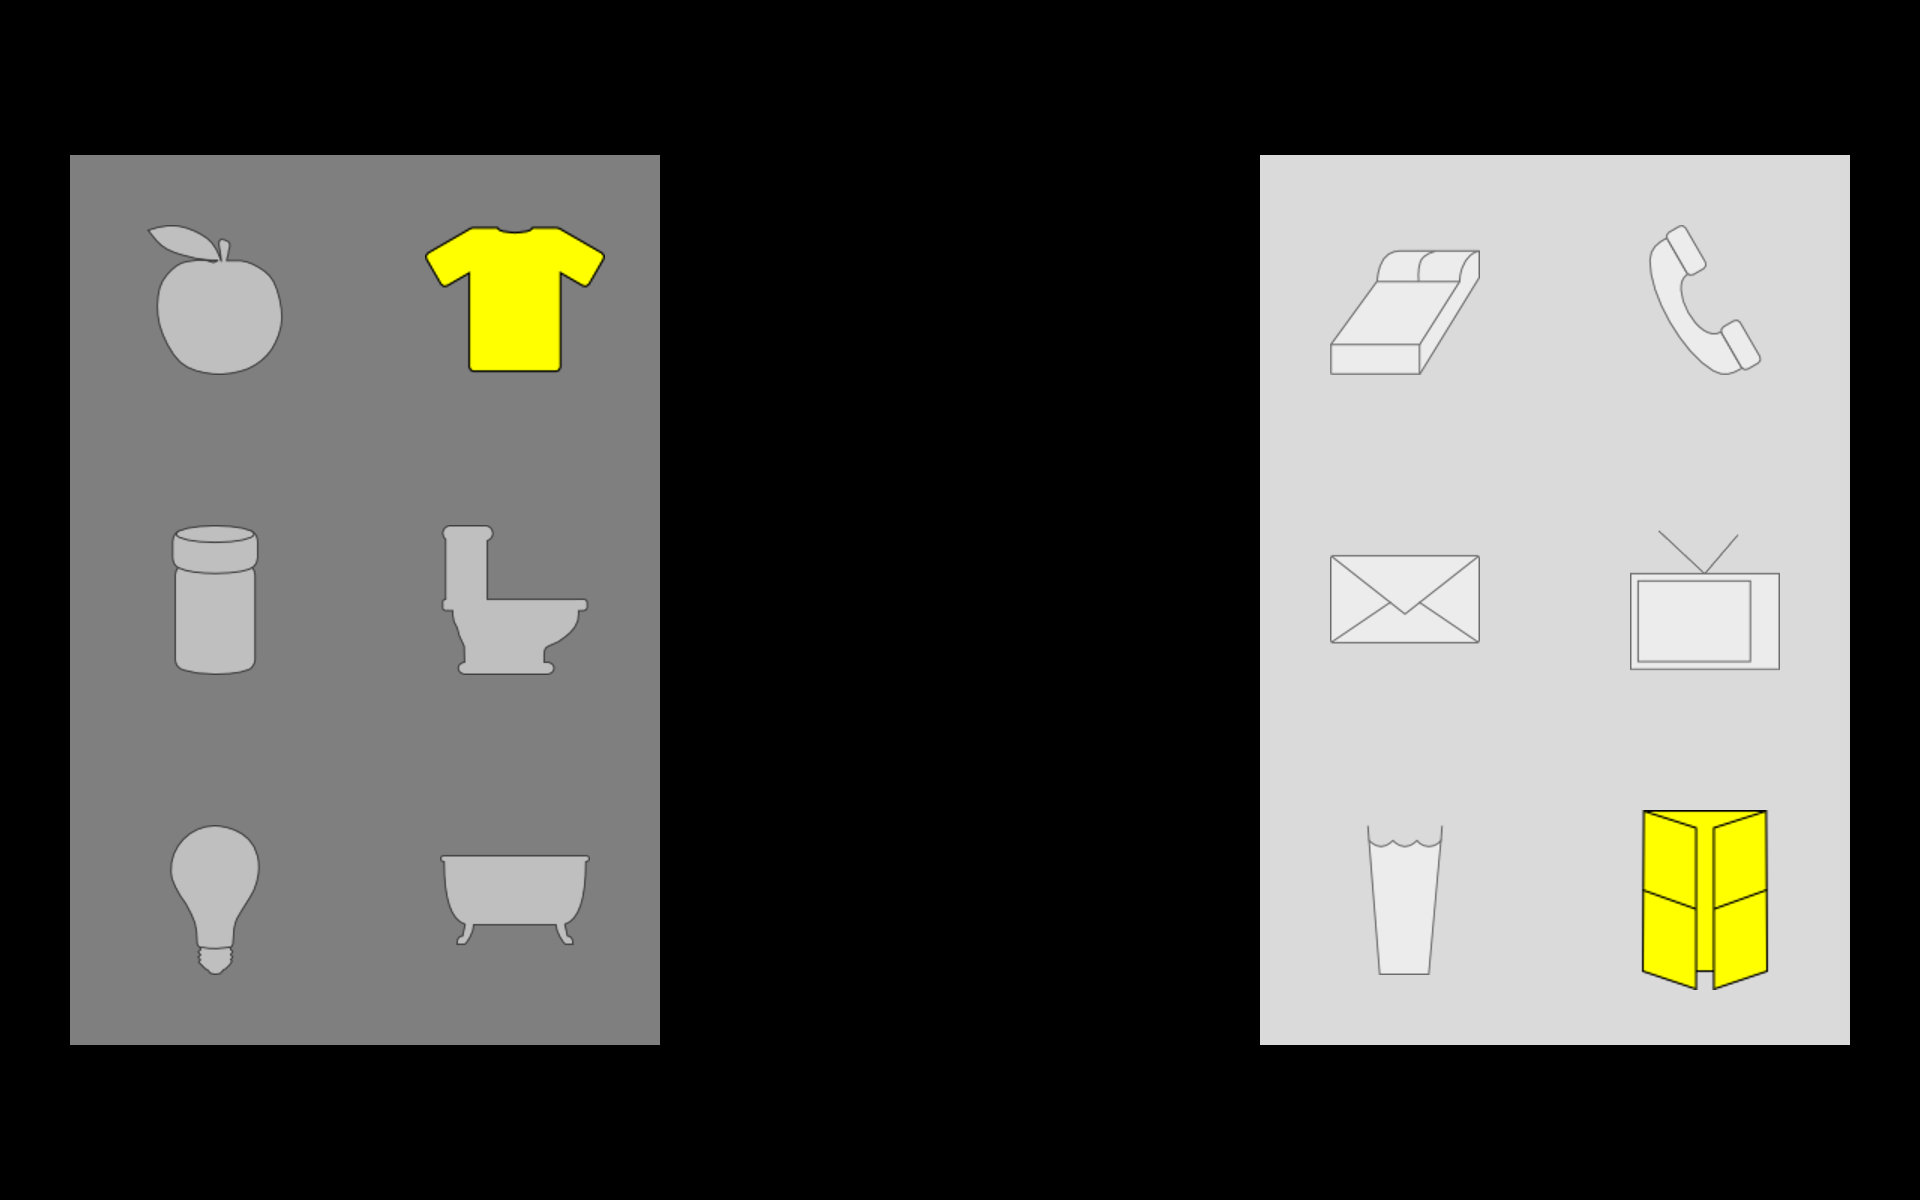
\includegraphics[width=0.5\textwidth]{pix/img0000332}
\caption{example of stimulus}
\label{fig:stim2oddball}
\end{figure}

%-------------------------------------------------------------------------------------------------------------------
%
%-------------------------------------------------------------------------------------------------------------------
\begin{figure}[t]
\centering
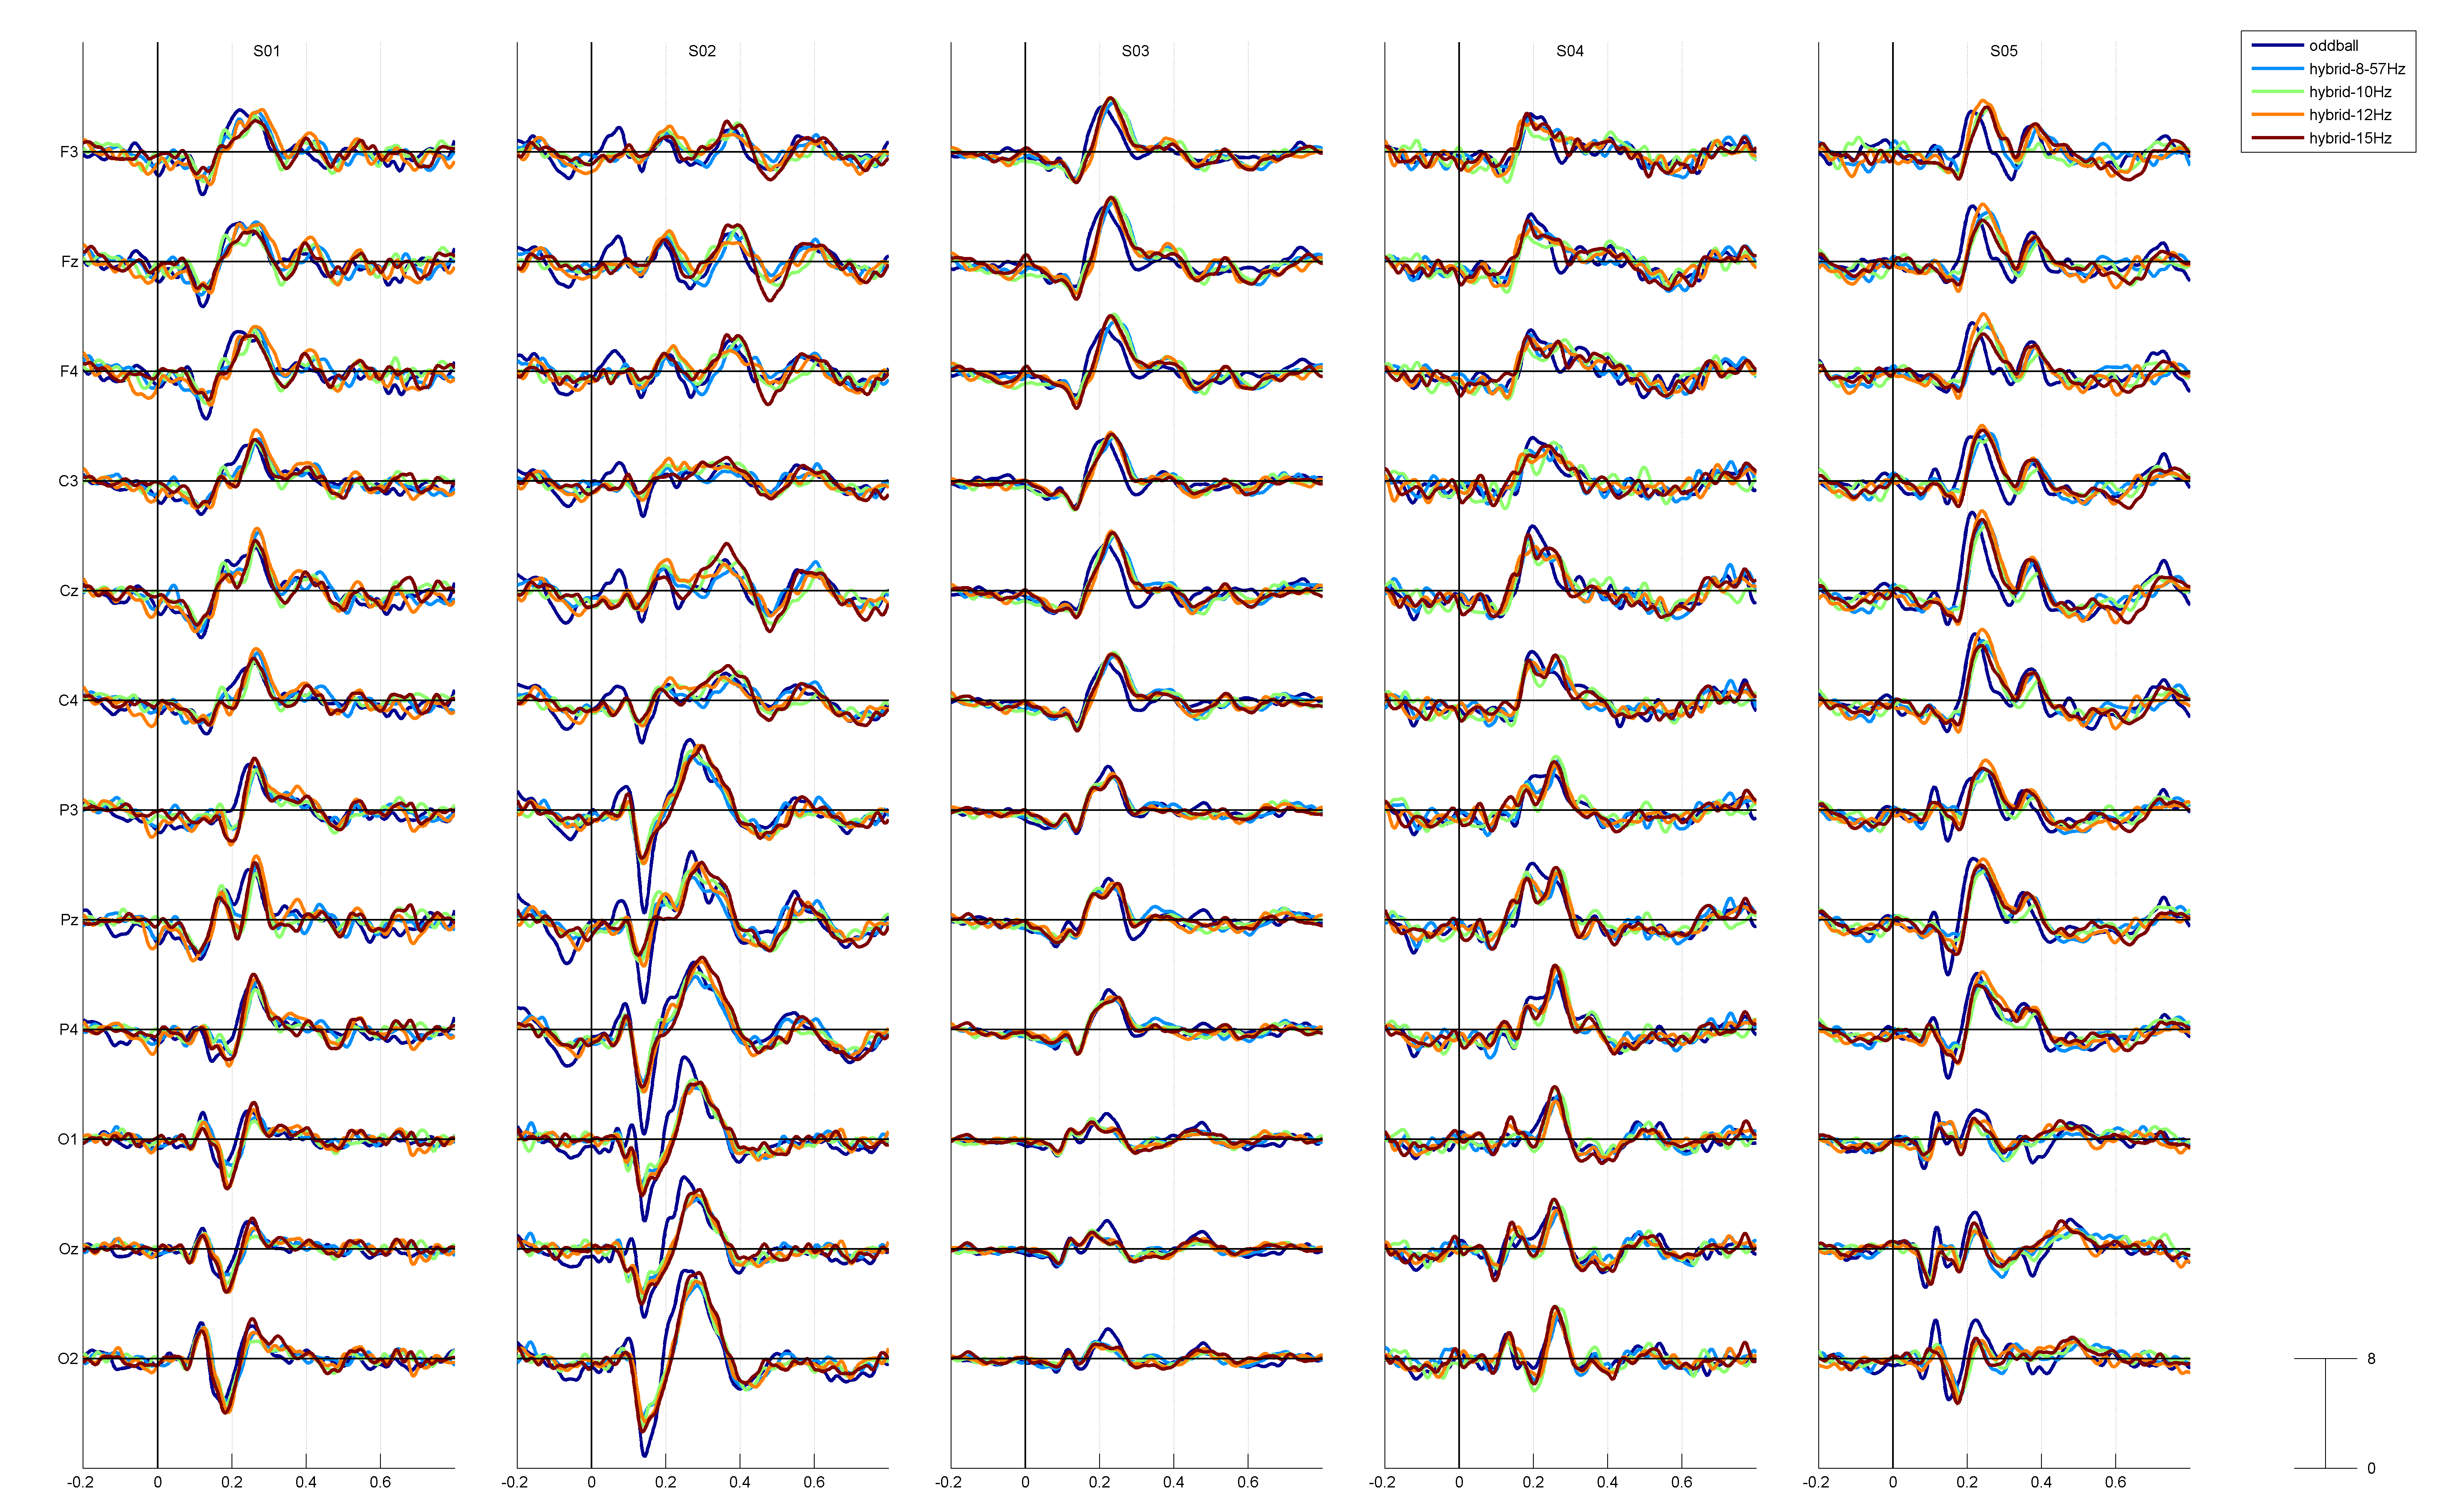
\includegraphics[width=\textwidth]{pix/targetERPs_1}
\caption{Average ERP responses to the target stimuli for a selection of EEG channels covering the scalp from frontal to occipital locations for all 5~experimental conditions for subjects S01 to S05. Time 0 represents the stimuli onset}
\label{fig:ERP_1}
\end{figure}


\begin{figure}[t]
\centering
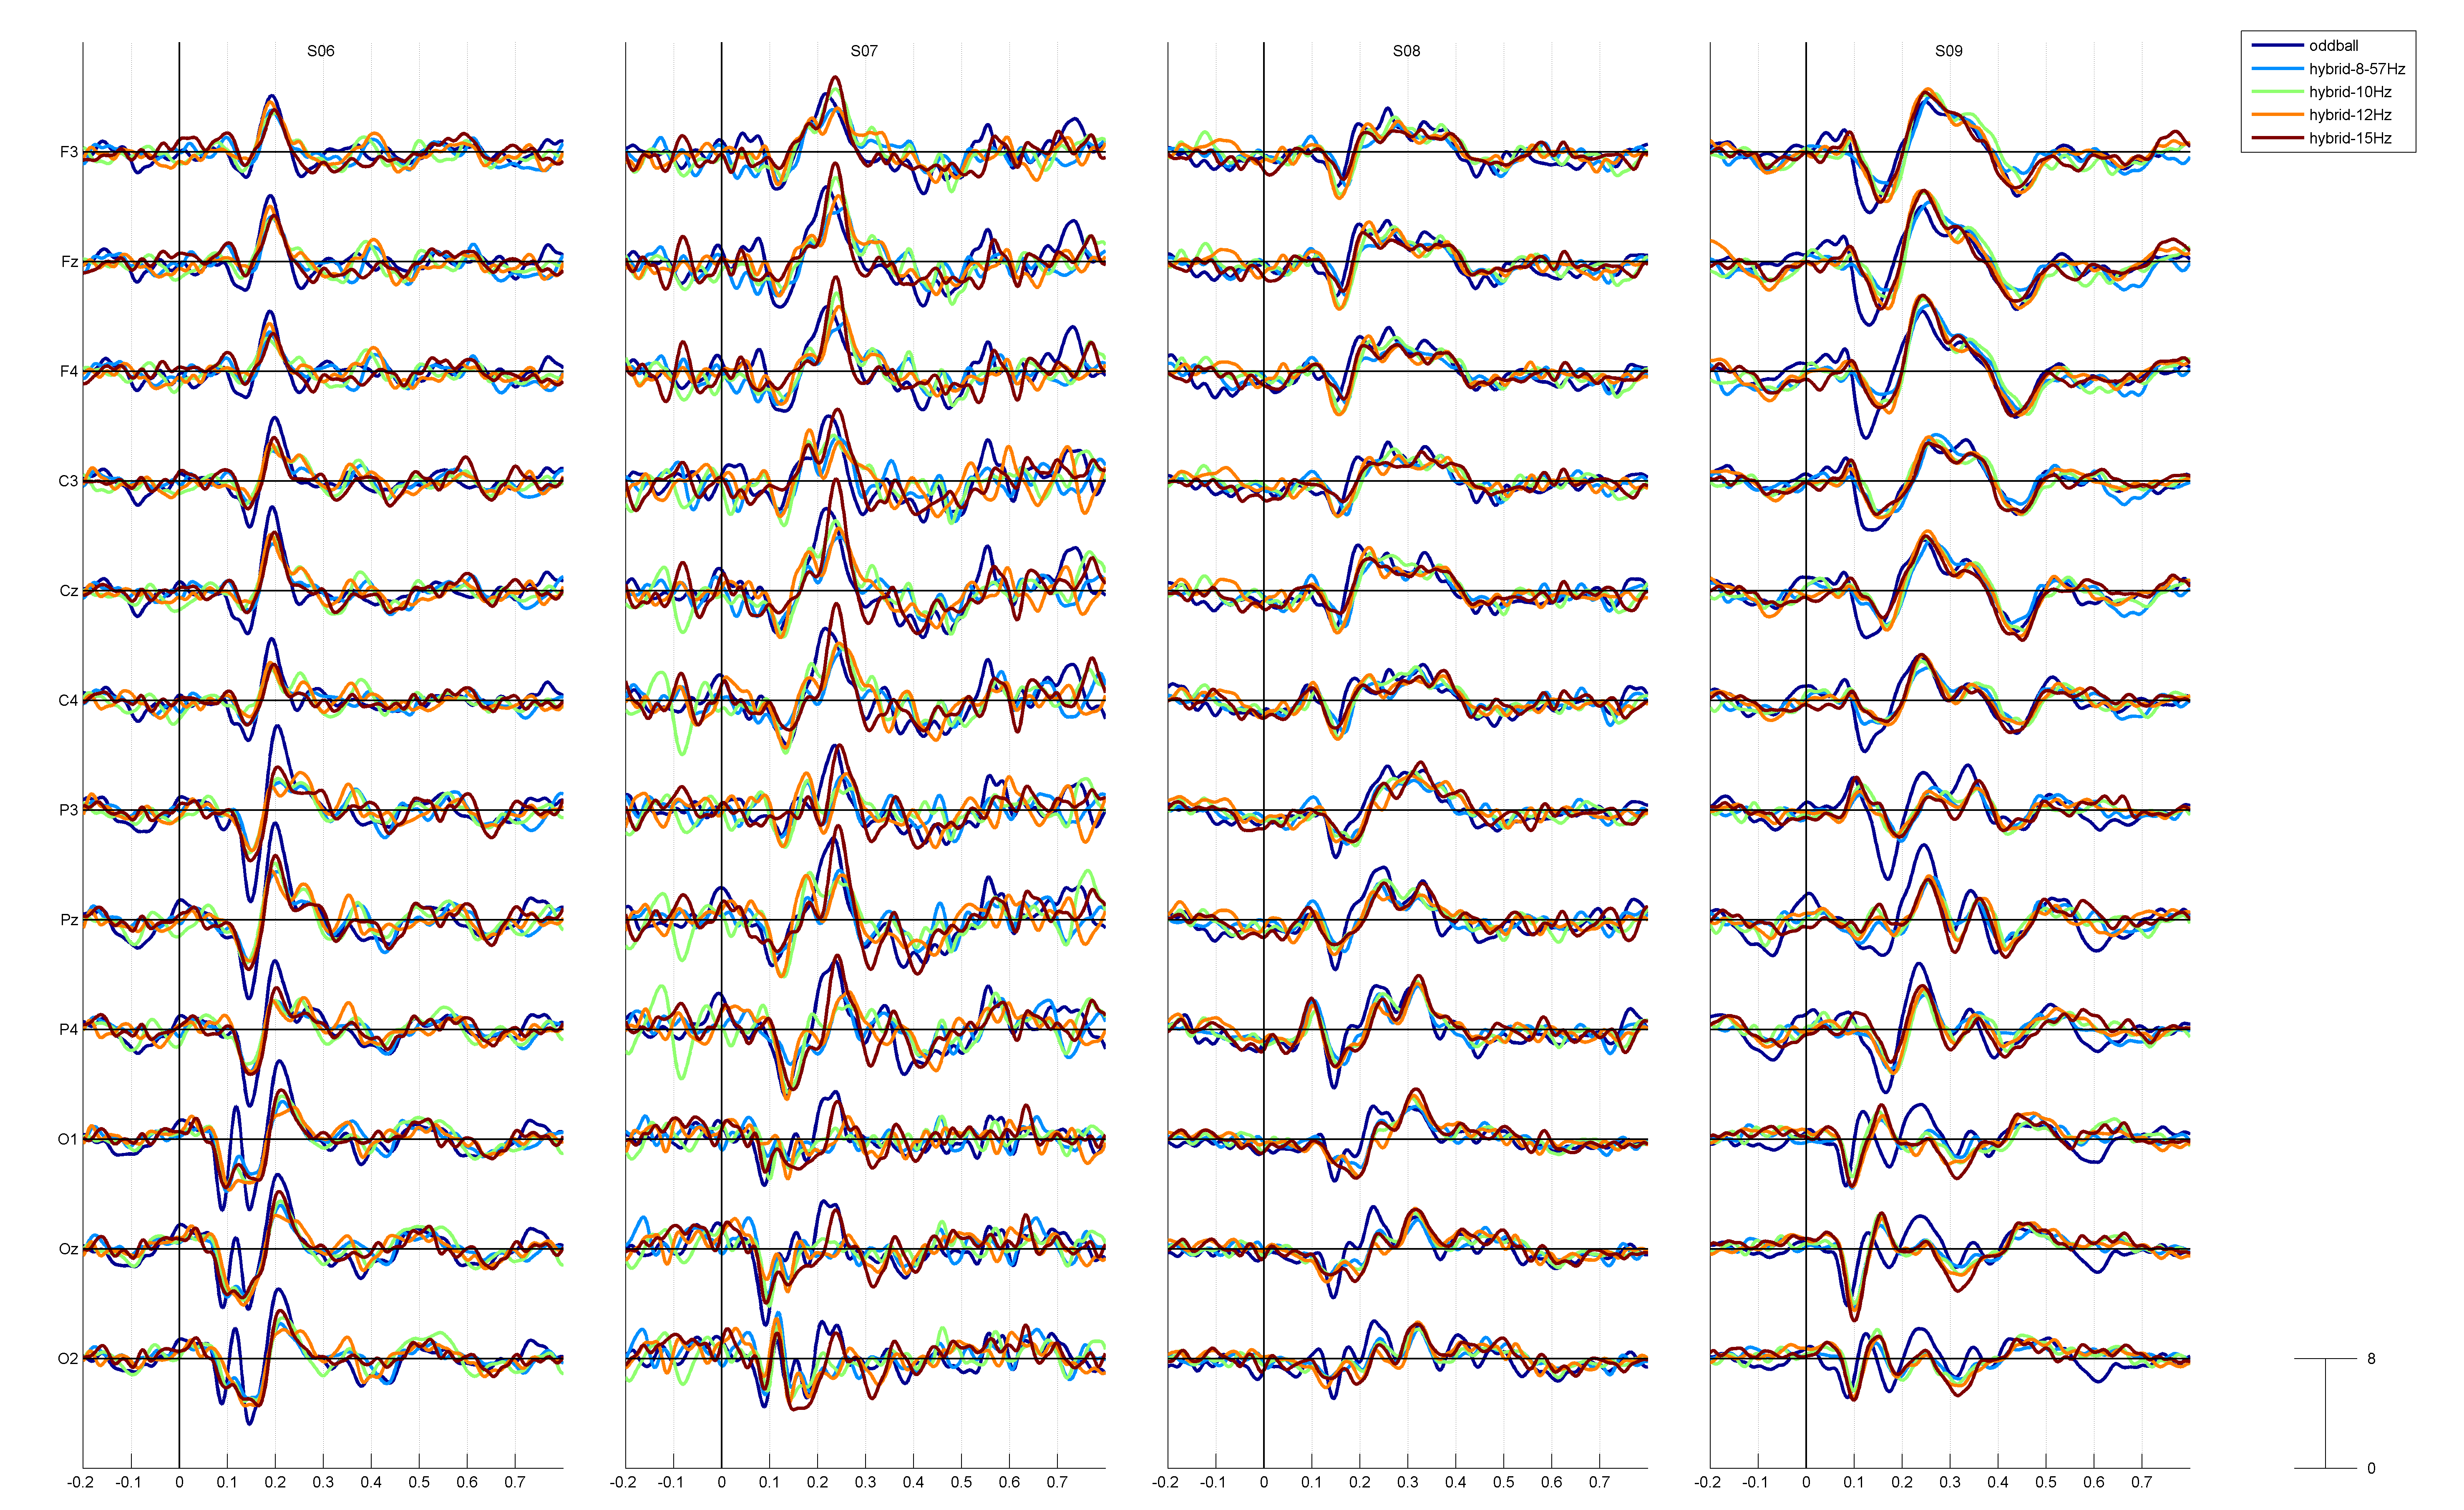
\includegraphics[width=\textwidth]{pix/targetERPs_2}
\caption{Average ERPs responses to the target stimuli for a selection of EEG channels covering the scalp from frontal to occipital locations for all 5~experimental conditions for subjects S06 to S09. Time 0 represents the stimuli onset}
\label{fig:ERP_2}
\end{figure}

%-------------------------------------------------------------------------------------------------------------------
%
%-------------------------------------------------------------------------------------------------------------------
\begin{figure}[t]
\centering
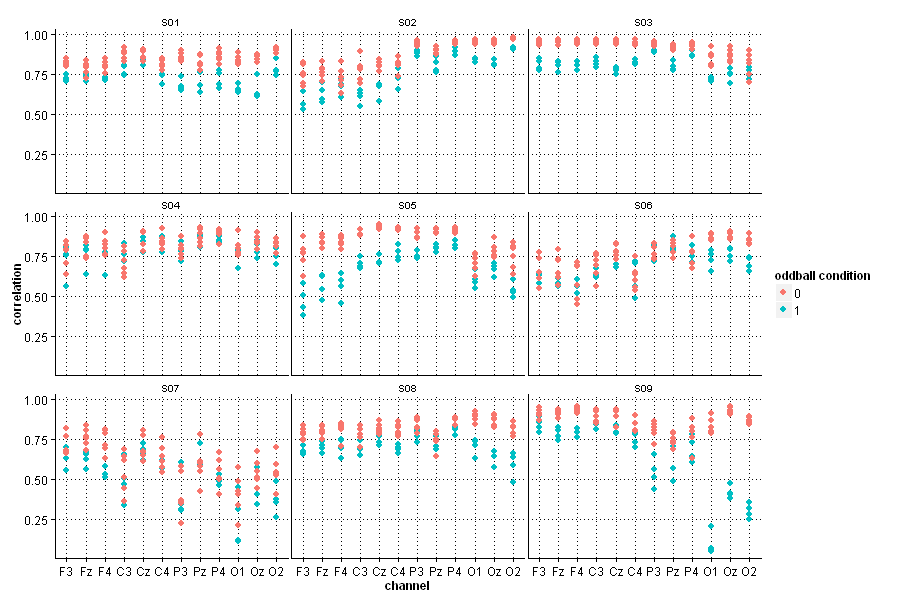
\includegraphics[width=\textwidth]{pix/correlationPoints}
\caption{
Pairwise correlations between ERPs for all condition per subject and EEG channel.
The blue dots represent correlation values measures between the average ERP recorded in the oddball condition and the average ERP recorded in each of the 4~hybrid conditions while the red dots represent correlation values measured between 2 average ERPs recorded in different hybrid condition.
}
\label{fig:corrERP}
\end{figure}

%-------------------------------------------------------------------------------------------------------------------
%
%-------------------------------------------------------------------------------------------------------------------
\begin{figure}[t]
\centering
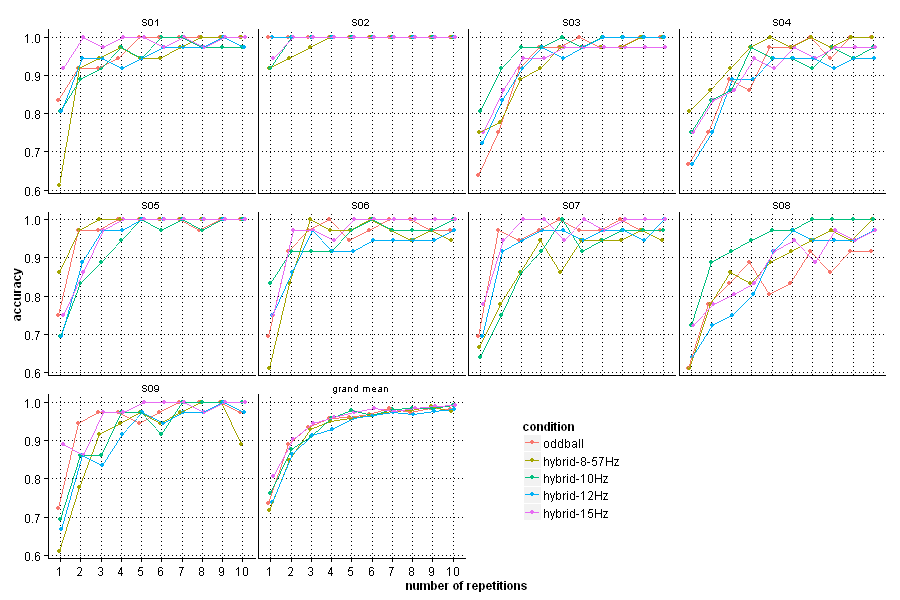
\includegraphics[width=\textwidth]{pix/P3Accuracy}
\caption{
Accuracy of oddball ERP detection with respect to the number of repetitions considered for each experimental condition, for each subject and averaged over subjects.
}
\label{fig:P3Acc}
\end{figure}

%-------------------------------------------------------------------------------------------------------------------
%
%-------------------------------------------------------------------------------------------------------------------
%\begin{figure}[t]
%\centering
%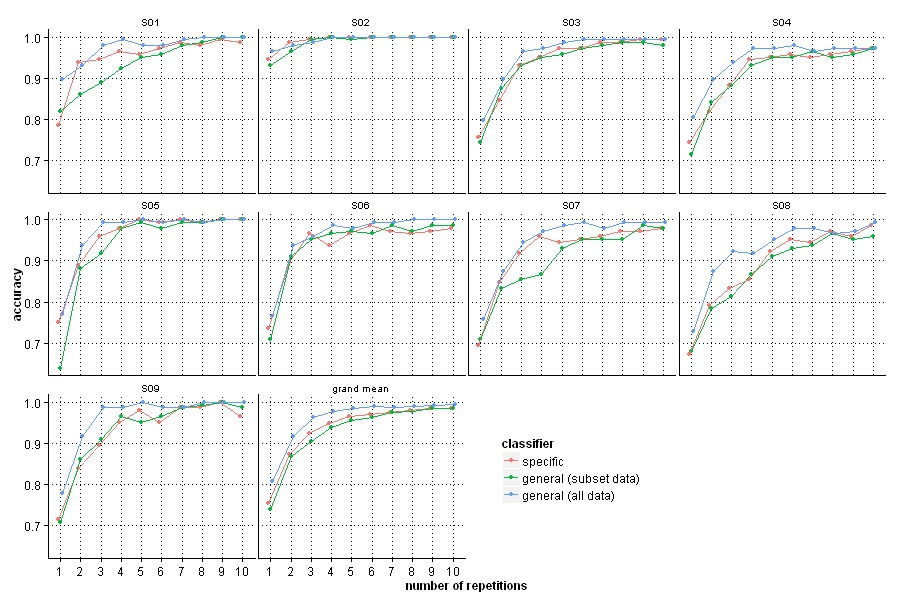
\includegraphics[width=\textwidth]{pix/P3AccuracyPerClassifierPerSubject}
%\caption{
%Accuracy of oddball ERP detection with respect to the number of repetitions considered for each experimental condition, for each subject and averaged over subjects.
%}
%\label{fig:P3AccPerClassifier}
%\end{figure}
\begin{figure}[t]
\centering
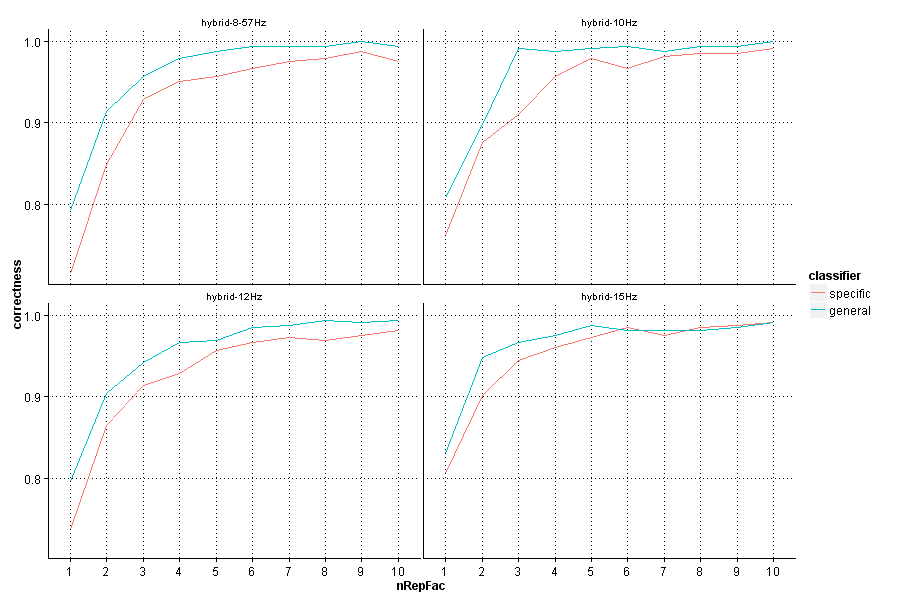
\includegraphics[width=\textwidth]{pix/P3AccuracyPerClassifierPerFreq}
\caption{
Accuracy of oddball ERP detection (subject mean) with respect to the number of repetitions considered for each experimental condition and classifier.
}
\label{fig:P3AccPerClassifier}
\end{figure}

%-------------------------------------------------------------------------------------------------------------------
%
%-------------------------------------------------------------------------------------------------------------------
\begin{figure}[t]
\centering
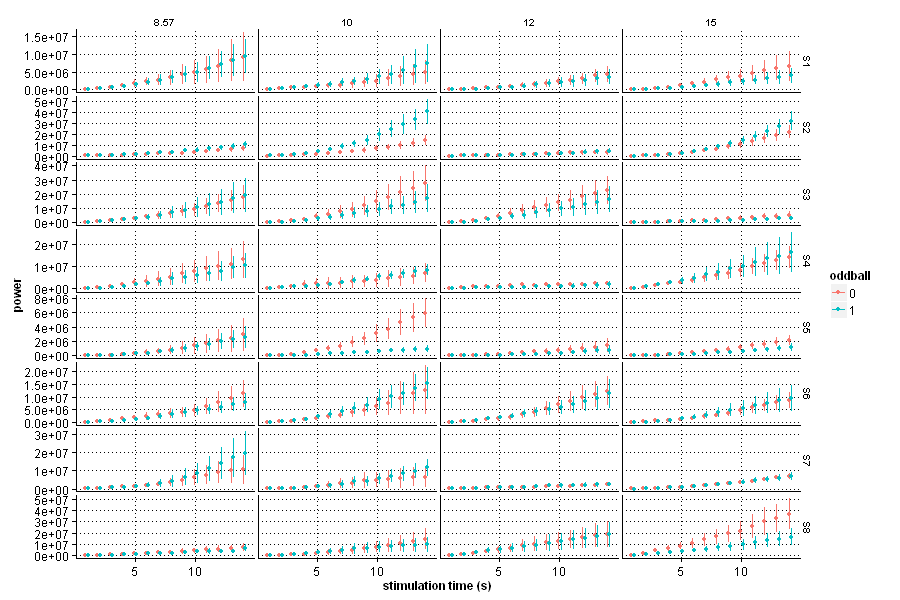
\includegraphics[width=\textwidth]{pix/meanPsdPlots}
\caption{
Power of the EEG signal recorded at Oz during the SSVEP stimulation with respect to the stimulation time for each subject, stimulation frequency and oddball condition.
The values are averaged over the 12~trials performed by each all subject in every conditions and the bars reprensent the $95\%$ confidence intervals.
}
\label{fig:meanPsd}
\end{figure}

%-------------------------------------------------------------------------------------------------------------------
%
%-------------------------------------------------------------------------------------------------------------------
\begin{figure}[t]
\centering
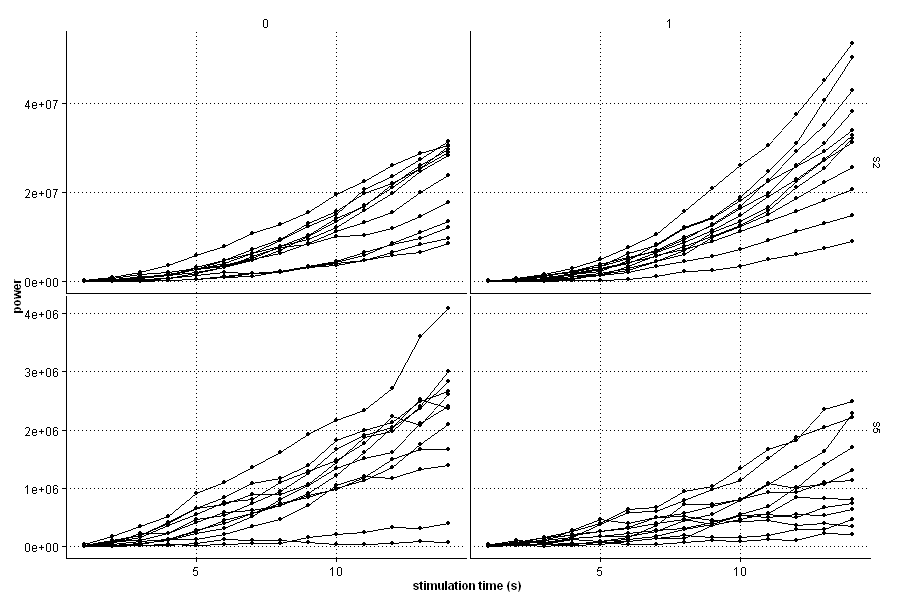
\includegraphics[width=\textwidth]{pix/psdPlotsAllTrials}
\caption{Power of the EEG signal recorded at Oz during the SSVEP stimulation with respect to the stimulation time for subjects S2 and S5, with a \SI{15}{\Hz} stimulation frequency with and with the oddball stimulation.
In each panel, all 12~trials are represented.
}
\label{fig:PsdAllTrials}
\end{figure}

%-------------------------------------------------------------------------------------------------------------------
%
%-------------------------------------------------------------------------------------------------------------------
\begin{figure}[t]
\centering
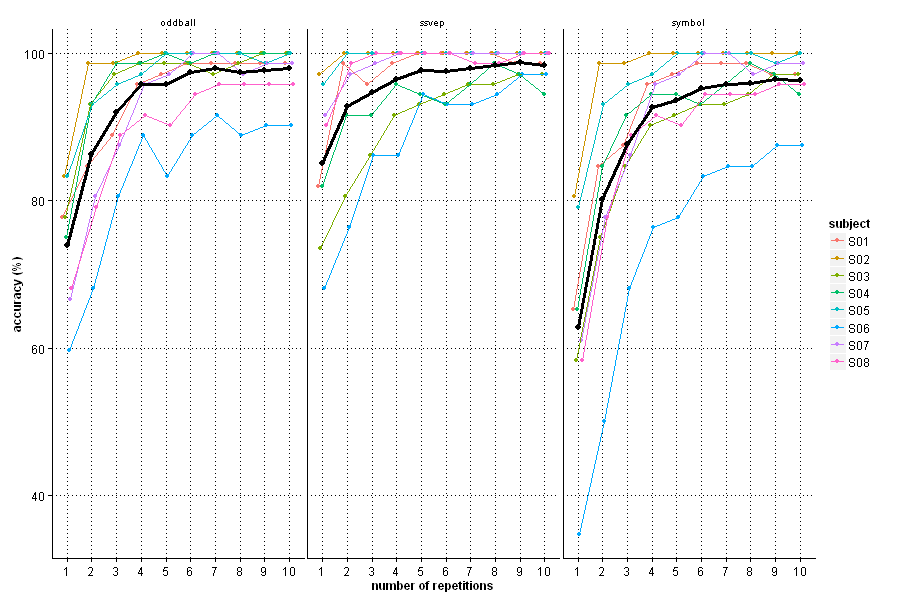
\includegraphics[width=\textwidth]{pix/exp3-acc}
\caption{
Detection accuracies with respect to the number of repetitions considered for each subject for the oddball ERP (left), SSVEP frequency (middle) and target symbol (left).
the black lines represent the average over subject.
One repetition of the stimulation cycle lasted for \SI{1.5}{\s}, the stimulation duration for a number $n_r$ of repetitions is thus $1.5 \times n_r$ seconds.
}
\label{fig:exp3-acc}
\end{figure}

%-------------------------------------------------------------------------------------------------------------------
%
%-------------------------------------------------------------------------------------------------------------------
\begin{figure}[t]
\centering
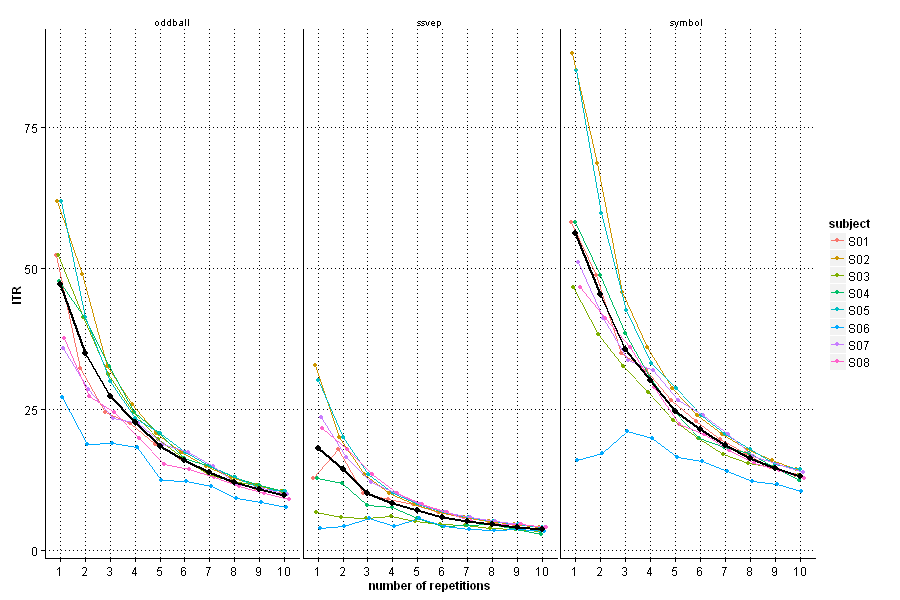
\includegraphics[width=\textwidth]{pix/exp3-ITR}
\caption{
ITR values with respect to the number of repetitions considered for each subject for the oddball ERP detection (left), SSVEP frequency detection (middle) and target symbol detection (right).
the black lines represent the average over subject.
One repetition of the stimulation cycle lasted for \SI{1.5}{\s}, the stimulation duration for a number $n_r$ of repetitions is thus $1.5 \times n_r$ seconds.
}
\label{fig:exp3-ITR}
\end{figure}


%-------------------------------------------------------------------------------------------------------------------
%
%-------------------------------------------------------------------------------------------------------------------
\begin{figure}[t]
\centering
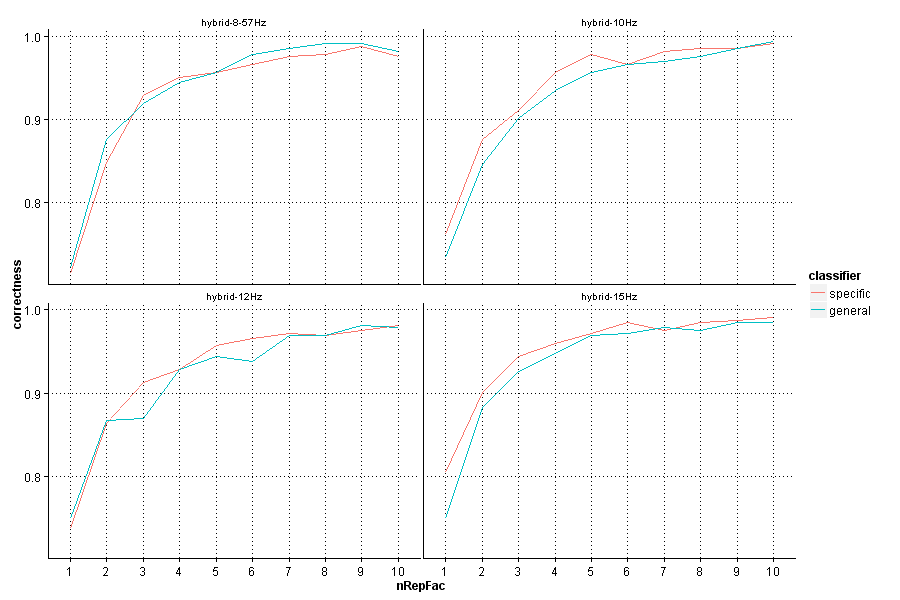
\includegraphics[width=\textwidth]{pix/P3AccuracyPerClassifierPerFreqSubset}
\caption{
Accuracy of oddball ERP detection (subject mean) with respect to the number of repetitions considered for each experimental condition and classifier.
}
\label{fig:P3AccPerClassifierSubset}
\end{figure}
